\subsection{Problem}

\renewcommand{\theequation}{\theenumi}
\begin{enumerate}[label=\thesection.\arabic*.,ref=\thesection.\theenumi]
\numberwithin{equation}{enumi}
\item  If A and B are events such that P(A/B) =
P(B/A), then
a) A  B but A , B
b) A = B
c) A  B = 
d) P(A) = P(B)
\\
\solution Since \begin{align}
P\brak{\frac{A}{B}} &= P\brak{\frac{B}{A}}\\
\frac{P\brak{A\cap B}}{P\brak{A}} &= \frac{P\brak{B\cap A}}{P\brak{B}}\\
\frac{P\brak{A\cap B}}{P\brak{A}} &= \frac{P\brak{A\cap B}}{P\brak{B}}\\
\frac{1}{P\brak{A}} &= \frac{1}{P\brak{B}}\\
\implies P\brak{A} &= P\brak{B}
\end{align}

\begin{comment}
	\begin{figure}[!ht]
	\centering
	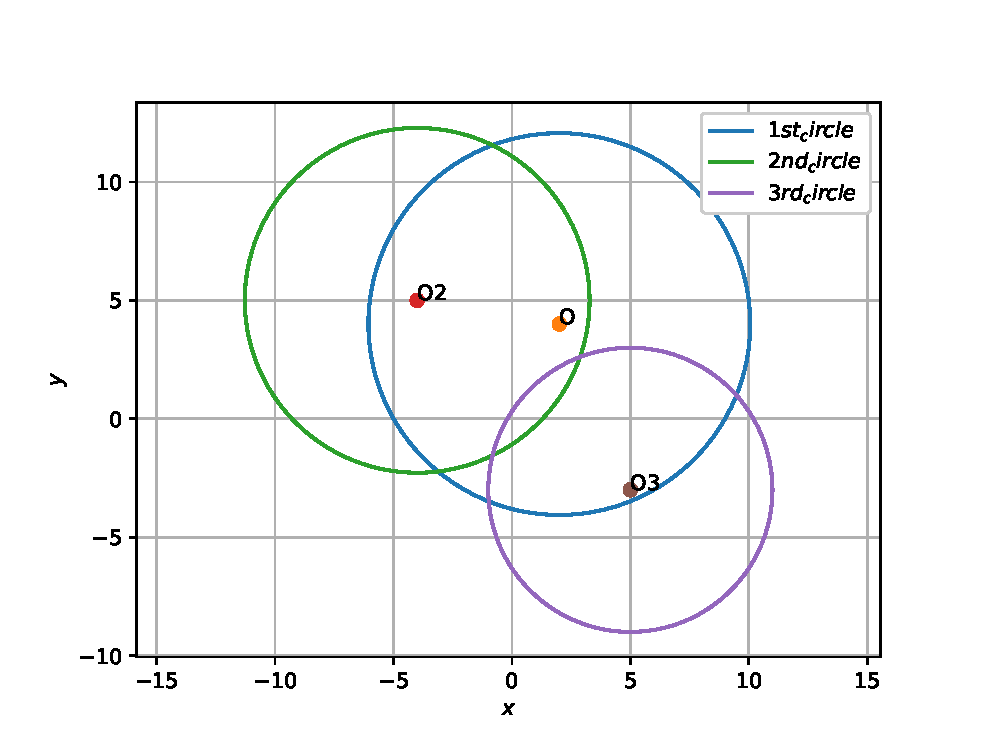
\includegraphics[width=\columnwidth]{./figs/circle/q18abc.eps}
	\caption{Circle of Q.4.2.5}
	\label{fig:qoeb}	
	\end{figure}
\end{comment}
\begin{comment}
	\begin{figure}[!ht]
	\centering
	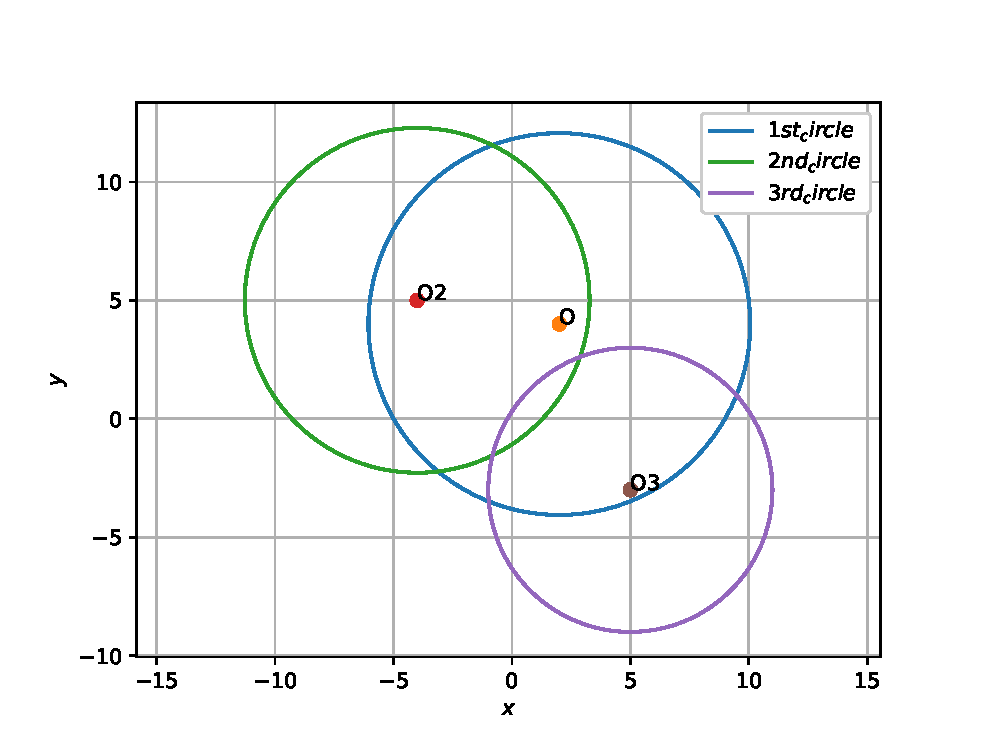
\includegraphics[width=\columnwidth]{./figs/circle/q18abc.eps}
	\caption{Circle of Q.4.2.5}
	\label{fig:qoec}	
	\end{figure}
\end{comment}
  
\end{enumerate}
